\documentclass[a4paper, 10.5pt]{jarticle}

\usepackage{txfonts}
\usepackage{bm}
\usepackage{boxedminipage}
\usepackage{multicol}
\usepackage[dvipdfmx]{graphicx}
\usepackage{listings}
\usepackage{subfigure}
\usepackage[dvipdfmx]{hyperref}
\usepackage{atbegshi}
\ifnum 42146=\euc"A4A2
\AtBeginShipoutFirst{\special{pdf:tounicode EUC-UCS2}}
\else
\AtBeginShipoutFirst{\special{pdf:tounicode 90ms-RKSJ-UCS2}}
\fi

\lstset{
  frame=single,
  breaklines = true,
  basicstyle=\small\ttfamily,
  numbers=left,
  numbersep=10pt,
  tabsize=1,
  extendedchars=true,
  xleftmargin=17pt,
  framexleftmargin=17pt
}

\setlength{\topmargin}{-20mm}
\setlength{\oddsidemargin}{-14mm}
\setlength{\textwidth}{180mm}
\setlength{\textheight}{260mm}

\makeatletter
\def\section{\@startsection{section}{1}{\z@}%
{1.75ex plus 0.5ex minus .2ex}{0.75ex plus .2ex}{\normalsize\bf}}
\def\subsection{\@startsection{subsection}{2}{\z@}%
{1.5ex plus 0.5ex minus .2ex}{0.5ex plus .2ex}{\normalsize\bf}}
\def\subsection{\@startsection{subsection}{3}{\z@}%
{1.0ex plus 0.5ex minus .2ex}{0.5ex plus .2ex}{\normalsize\bf}}
\makeatother
\renewcommand{\baselinestretch}{0.85}

\begin{document}

\begin{flushleft}
\textbf{{マルチメディア特論 レポート}}
\end{flushleft}
\begin{flushright}
2018/06/28 (金曜日)\par
理工学研究科 情報科学専攻\par
学籍番号 47018327\par
若林 秀和
\end{flushright}

\begin{quote}
\section{処理内容}
csvファイルを読み込み, X, Y, Zを切り出しそれぞれ配列に格納する. 各配列の合計を計算し, その値から白色点の座標を求める. また, 各配列を正規化し, 0〜1までの値に変更する. X, Yの値をプロットすると, 馬蹄型の曲線Sが出来る. 曲線の両端周辺の座標を求め, この二点を結ぶ直線(L)を求める. 白色点からSの各点まで直線で結び, この直線をN分割する(今回はN=300). そして, 分割した点のx座標, y座標を, 記録用の配列に格納する. また, 白色点からLの格点まで直線で結び, この直線をN分割する. 同様に, 分割した点のx座標, y座標を同じ配列に格納する. これにより, 馬蹄型の内部の点の座標を求めることが出来る. 次に, 各点のx,y座標からRGBの値を計算する. X,Y,Zに関しては, 文献\cite{col} にある計算を使い求め, 問題文にあった変換行列を使いRGBを計算する. そして, 計算したRGBを配列に格納する. 最後に, 求めたxy座標とRGBの配列で散布図を作成する.

\section{実行環境}
\begin{itemize}
  \item ubuntu16.04
  \item Python 2.7.12
  \item 実行コマンド: \$python color.py
\end{itemize}

\section{結果}
実行結果を図\ref{res}に示す. パラメータを変更することで, 白色部分の幅や, 明るさを調整することが出来る.

\begin{figure}[htbp]
  \center
  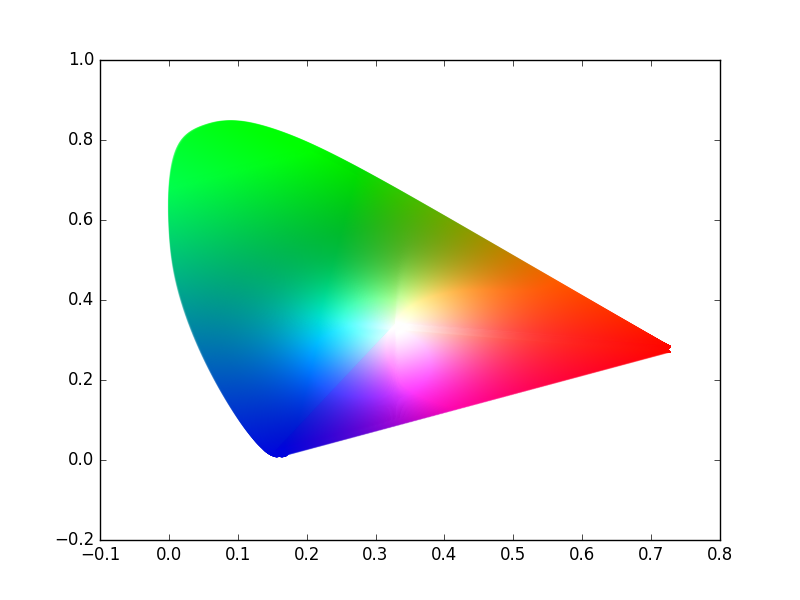
\includegraphics[scale = 0.38]{figure.png}
  \caption{xy色度図}
  \label{res}
\end{figure}

\begin{thebibliography}{99}
  \bibitem{col}
  犬井正男: ``色度図の着色,'' 東京工芸大学工学部紀要, Vol.\ 36 No.\ 1 (2013)
\end{thebibliography}

\end{quote}
\end{document}
